\documentclass[submission,copyright,creativecommons]{eptcs}
\providecommand{\event}{LFMTP 2022} % Name of the event you are submitting to
%\usepackage{breakurl}             % Not needed if you use pdflatex only.
\usepackage{underscore}           % Only needed if you use pdflatex.

\title{An Implementation of Set Theory with Pointed Graphs in Dedukti}
\author{Valentin Blot
\institute{Inria, France\\
LMF, ENS Paris-Saclay, France}
\email{valentin.blot@inria.fr}
\and
Gilles Dowek
\institute{Inria, France\\
LMF, ENS Paris-Saclay, France}
\email{gilles.dowek@ens-paris-saclay.fr}
\and
Thomas Traversié
\institute{CentraleSupélec, France}
\email{thomas.traversie@inria.fr}
}

\def\titlerunning{An Implementation of Set Theory with Pointed Graphs in Dedukti}
\def\authorrunning{V. Blot, G. Dowek, T. Traversié}

%% My packages

\usepackage{tikz}
\usepackage{url}
\usepackage[utf8]{inputenc}
\usepackage[T1]{fontenc}

%% Lambdapi code

\usepackage{listings}
\usepackage{amssymb}
\usepackage{mathtools}
\usepackage{xcolor}
\definecolor{green}{RGB}{0,130,0}
\definecolor{lightgrey}{RGB}{240,240,240}

\lstdefinelanguage{Lambdapi}
{
  inputencoding=utf8,
  extendedchars=true,
  numbers=none,
  numberstyle={},
  tabsize=2,
  basicstyle={\ttfamily\upshape\mdseries},
  backgroundcolor=\color{lightgrey},
  keywords={abort,admit,admitted,apply,as,assert,assertnot,associative,assume,begin,builtin,commutative,compute,constant,debug,end,fail,flag,focus,generalize,have,in,induction,inductive,infix,injective,left,let,notation,off,on,opaque,open,prefix,print,private,proofterm,protected,prover,prover_timeout,quantifier,refine,reflexivity,require,rewrite,right,rule,sequential,simplify,solve,symbol,symmetry,type,TYPE,unif_rule,verbose,why3,with},
  sensitive=true,
  keywordstyle=\color{blue},
  morecomment=[l]{//},
  commentstyle={\itshape\color{red}},
  string=[b]{"},
  stringstyle=\color{orange},
  showstringspaces=false,
  literate=
  {↪}{$\hookrightarrow$}1
  {→}{$\rightarrow$}1
  {Π}{$\Pi$}1
  {≔}{\quad $\coloneqq$}1
  {𝔹}{$\mathbb{B}$}1
  {𝕃}{$\mathbb{L}$}1
  {ℕ}{$\mathbb{N}$}1
  {α}{$\alpha$}1
  {λ}{$\lambda$}1
  {σ}{$\sigma$}1
  {π}{$\pi$}1
  {τ}{$\tau$}1
  {ω}{$\omega$}1
  {∧}{$\wedge$}1
  {∨}{$\vee$}1
  {≤}{$\le$}1
  {≠}{$\neq$}1
  {∉}{$\notin$}1
  {×}{$\times$}1
  {ρ}{$\rho$}1
  {∈}{$\in$}1
  {∀}{$\forall$}1
  {∃}{$\exists$}1
  {⇒}{$\Rightarrow$}1
  {⇔}{$\Leftrightarrow$}1
  {⊤}{$\top$}1
  {⊥}{$\bot$}1
}
\lstset{language={Lambdapi}}

%% Macro

\def\Type{\mbox{\tt TYPE}}
\def\Kind{\mbox{\tt KIND}}
\def\ra{\rightarrow}
\def\lra{\longrightarrow}
\def\Set{\mbox{\it Set}}
\def\bliota{{ind}}
\def\El{{\mbox{\it El}}}
\def\Prop{{\mbox{\it Prop}}}
\def\imp{\mathbin{\Rightarrow}}
\def\fa{{\forall}}
\def\bltop{{\top}}
\def\blbot{{\bot}}
\DeclareMathOperator{\blneg}{{\neg}}
\def\conj{\mathbin{\wedge}}
\def\disj{\mathbin{\vee}}
\def\ex{{\exists}}

\newtheorem{theorem}{Theorem}[section]

\newenvironment{proof}{\noindent {\em Proof.}}{\medskip}

\newcommand{\dedukti}{\textsc{Dedukti}}
\newcommand{\lpcm}{$\lambda \Pi\textit{-calculus modulo theory}$}

\def\Graph{{\mbox{\it Graph}}}
\def\Node{{\mbox{\it Node}}}
\def\omicron{{\mbox{\it omicron}}}
\def\arr{{\mbox{\it arrow}}}

%%%%%%%%%%%%

\begin{document}
\maketitle

\begin{abstract}
\dedukti ~is a type-checker for the \lpcm, a logical framework that allows the extension of conversion with user-defined rewrite rules. In this paper, we present the implementation of a version of Dowek-Miquel's intuitionistic set theory in \dedukti. To do so, we adapt this theory -- based on the concept of pointed graphs -- from \textit{Deduction modulo theory} to \lpcm, and we \textit{formally} write the proofs in \dedukti. In particular, this implementation requires the definition of a deep embedding of a certain class of formulas, as well as its interpretation in the theory.
\end{abstract}

\section{Introduction}

During the last decades, theorem provers have attracted a lot of interest from various fields of science. Especially, the use of such tools has become more and more common in the areas of software verification and formalization of mathematics. As an example, verification has become mandatory for software running on aircrafts, and formalization of mathematical results allowed the scientific community to trust some complicated proofs of recent results, as well as identify and fix errors in some cases.

This growing interest has triggered the developement of many theorem provers, with various focuses and based on a large range of theories. While the diversity of theorem provers provides users with a wide range of tools, this comes at the expense of a lack of interaction and reusability between proof fragments done in different tools. The \lpcm ~is a logical framework supporting dependent types and user-definable rewrite rules, and \dedukti ~\cite{expressing} is a type-checker for this framework. The definition of well-chosen rewrite rules allows the encoding of various logics, and hence the translations between various theorem provers through the \dedukti ~tool.

Several theorem provers, such as \textsc{Mizar}, \textsc{Atelier B} and \textsc{Isabelle/ZF}, are based on set theory. In order to extend the interoperability allowed by \dedukti ~to these provers, it is necessary to encode set theory in the \lpcm, and to implement this encoding in \dedukti. The goal of this paper is to present such an encoding and implementation. In order to facilitate the proof of its correctness, we implement this encoding in the tool \textsc{Lambdapi} that provides tactics to help the user in the production of proofs type-checkable in \dedukti.

Stating each axiom of set theory in \dedukti ~would lead to an implementation that does not satisfy a cut-elimination theorem. In particular, it would forbid extraction of witnesses from constructive existence proofs.

An alternative option would be to orient these axioms as rewriting rules. For instance the powerset axiom $x \in \mathcal{P}(y) \Leftrightarrow x \subseteq y$ would be replaced with the rewrite rule $x \in \mathcal{P}(y) \lra x \subseteq y$. However, as pointed out by Crabbé~\cite{crabbe}, such a formulation of set theory does not satisfy a cut-elimination property either. Indeed, if for a given set $a$ we define the set $b\equiv\{x\in a\,|\,x\in x\}$ then $b\in b$ would get rewritten to $b\in a\wedge b\in b$, leading to an infinite reduction.

In the current paper, we represent sets as \textit{pointed graphs} \cite{pointed}. With such a formulation, we can prove a cut-elimination theorem: for every proof in natural deduction there exists a cut-free proof of the same statement. Such an encoding of set theory has been defined in the context of \textit{Deduction modulo theory}~\cite{zermodulo}, together with pencil and paper proofs. At that time, the \lpcm ~had not been defined yet, and the first contribution of the current paper is to adapt this encoding to the \lpcm. In particular, we avoid the original definition of classes of nodes by using the quantification on propositions permitted by \lpcm. This reduces the size of the signature from 31 to 26 symbols.

The second contribution consists in the implementation of this new theory in \dedukti. In the original formulation of the theory some lemmas are only valid for a specific class of formulas, as their proofs proceed by induction on the structure of these formulas. Implementing these lemmas in \dedukti ~requires the definition of an inductive sort of formulas together with an interpretation of these formulas into the general type of propositions. This interpretation is defined with rewriting rules. The current development is the first, to our knowledge, to use such a reflection principle defined with rewriting rules in \dedukti. The generality of this method still remains to be investigated.

\section{The Theory of Pointed Graphs}

The set theory with pointed graphs developed by Dowek and Miquel is called Intuitionistic Zermelo set theory in \textit{Deduction modulo} (IZmod). We give here an informal presentation of the ideas developed in \cite{zermodulo}.

\subsection{Sets as Pointed Graphs}

\label{informal}

In the IZmod theory, sets are represented by pointed graphs, that is, direct graphs with a distinguished node: the root. We give here the representation of several sets as pointed graphs. The root is indicated by the filled circle. The location of the root is important as it changes the set represented by the pointed graph, distinct pointed graphs represent the same set. For example, in the third graph, the node $b$ is irrelevant since the root is $c$.

\begin{figure}[h]
\centering
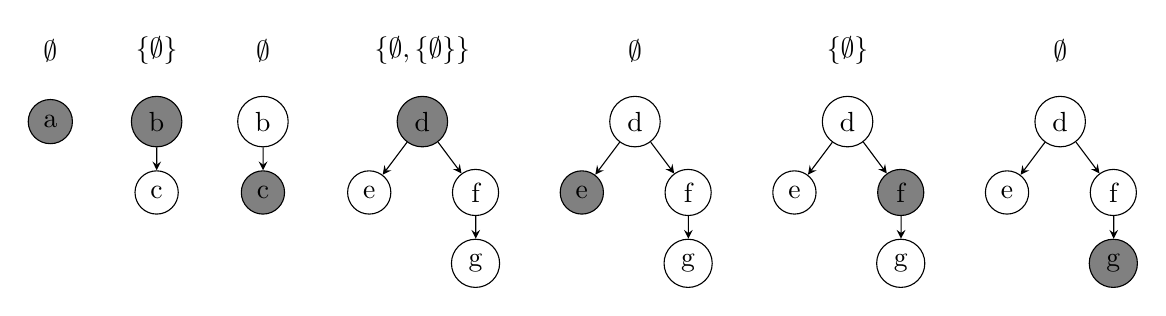
\begin{tikzpicture}[>=stealth,yscale=1.8,xscale=1.35]  

\node(h1) at (3,3.5)[text centered]{$\emptyset$};
\node(a) at (3,3)[circle,draw,text centered,fill=gray] {a};
\node(h2) at (4,3.5)[text centered]{$\{\emptyset\}$};
\node(b) at (4,3)[circle,draw,text centered,fill=gray] {b};
\node(c) at (4,2.5)[circle,draw,text centered] {c};
\node(h3) at (5,3.5)[text centered]{$\emptyset$};
\node(b1) at (5,3)[circle,draw,text centered] {b};
\node(c1) at (5,2.5)[circle,draw,text centered,fill=gray] {c};
\node(h3) at (6.5,3.5)[text centered]{$\{\emptyset,\{\emptyset\}\}$};
\node(d) at (6.5,3)[circle,draw,text centered,fill=gray] {d};
\node(e) at (6,2.5)[circle,draw,text centered] {e};
\node(f) at (7,2.5)[circle,draw,text centered] {f};
\node(g) at (7,2)[circle,draw,text centered] {g};
\node(h4) at (8.5,3.5)[text centered]{$\emptyset$};
\node(d1) at (8.5,3)[circle,draw,text centered] {d};
\node(e1) at (8,2.5)[circle,draw,text centered,fill=gray] {e};
\node(f1) at (9,2.5)[circle,draw,text centered] {f};
\node(g1) at (9,2)[circle,draw,text centered] {g};
\node(h5) at (10.5,3.5)[text centered]{$\{\emptyset\}$};
\node(d2) at (10.5,3)[circle,draw,text centered] {d};
\node(e2) at (10,2.5)[circle,draw,text centered] {e};
\node(f2) at (11,2.5)[circle,draw,text centered,fill=gray] {f};
\node(g2) at (11,2)[circle,draw,text centered] {g};
\node(h6) at (12.5,3.5)[text centered]{$\emptyset$};
\node(d3) at (12.5,3)[circle,draw,text centered] {d};
\node(e3) at (12,2.5)[circle,draw,text centered] {e};
\node(f3) at (13,2.5)[circle,draw,text centered] {f};
\node(g3) at (13,2)[circle,draw,text centered,fill=gray] {g};
                      
\draw[->] (b) -- (c); 
\draw[->] (b1) -- (c1); 
\draw[->] (d) -- (e);
\draw[->] (d) -- (f);
\draw[->] (f) -- (g);
\draw[->] (d1) -- (e1);
\draw[->] (d1) -- (f1);
\draw[->] (f1) -- (g1);
\draw[->] (d2) -- (e2);
\draw[->] (d2) -- (f2);
\draw[->] (f2) -- (g2);
\draw[->] (d3) -- (e3);
\draw[->] (d3) -- (f3);
\draw[->] (f3) -- (g3);

\end{tikzpicture}
\end{figure}

IZmod has a sort of pointed graphs and a sort of nodes. If $a$ is a pointed graph, $root(a)$ is the root of $a$, which is a node. If $x$ is a node of $a$, then $a/x$ denotes the pointed graph $a$ where the root has been replaced with $x$. If $y$ is also a node of $a$, $x~\eta_a~y$ is the proposition asserting that there is a edge in $a$ from $y$ to $x$. Following this interpretation, IZmod contains the following rewriting rules:
$$ x \ \eta_{a/z} \ y \longrightarrow x \ \eta_a \ y \qquad\qquad root(a/x) \longrightarrow x \qquad\qquad (a/x)/y \longrightarrow a/y $$

As noted above, distinct pointed graphs can represent the same set. Two pointed graphs representing the same set are related through a notion of bisimilarity, denoted $\simeq$, and defined with the rewrite rule:

\begin{equation*}
\begin{split}
a \simeq b \lra~\ex r,~ &r~root(a)~root(b) \\
&\conj \ \fa x \fa x'~\fa y~(x'~\eta_a~x~\conj~r~x~y~\imp~\ex y'~(y'~\eta_b~y~\conj~r~x'~y')) \\
&\conj \ \fa y \fa y'~\fa x~(y'~\eta_b~y~\conj~r~x~y~\imp~\ex x'~(x'~\eta_a~x~\conj~r~x'~y')))
\end{split}
\end{equation*}

As an example, the following pointed graphs are bisimilar, hence they represent the same set:

\begin{figure}[h]
\centering
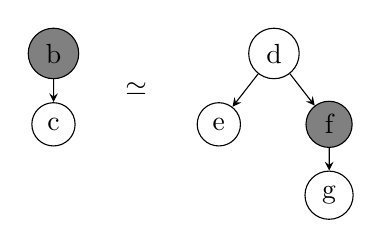
\begin{tikzpicture}[>=stealth,yscale=1.8,xscale=1.4]  

\node(b) at (5,3)[circle,draw,text centered,fill=gray] {b};
\node(c) at (5,2.5)[circle,draw,text centered] {c};
\node(d) at (7,3)[circle,draw,text centered] {d};
\node(e) at (6.5,2.5)[circle,draw,text centered] {e};
\node(f) at (7.5,2.5)[circle,draw,text centered,fill=gray] {f};
\node(g) at (7.5,2)[circle,draw,text centered] {g};
\node(h) at (5.75,2.75)[text centered]{$\simeq$};
                      
\draw[->] (b) -- (c); 
\draw[->] (d) -- (e);
\draw[->] (d) -- (f);
\draw[->] (f) -- (g);

\end{tikzpicture}
\end{figure}

In set theory, there only exists one sort: the sets. The IZmod theory has two sorts: nodes and pointed graphs, and two notions related to set membership: relations between pointed graphs and relations between nodes within the same graph. As an example, take $\emptyset \in \{\emptyset\}$:

\begin{figure}[h]
\centering
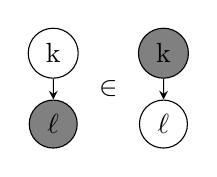
\begin{tikzpicture}[>=stealth,yscale=1.8,xscale=1.4]  

\node(d) at (6,3)[circle,draw,text centered] {k};
\node(e) at (6,2.5)[circle,draw,text centered,fill=gray] {$\ell$};
\node(k) at (6.5,2.75)[text centered]{$\in$};
\node(f) at (7,3)[circle,draw,text centered,fill=gray] {k};
\node(g) at (7,2.5)[circle,draw,text centered] {$\ell$};
                      
\draw[->] (d) -- (e);
\draw[->] (f) -- (g);

\end{tikzpicture}
\end{figure}

Since there is an edge from $k$ to $\ell$, the set represented by the pointed graph with root $\ell$ is an element of the set represented by the pointed graph with root $k$. But any pointed graph bisimilar to the pointed graph with root $\ell$ also represents a set that is an element of the set represented by the pointed graph with root $k$. This leads to the definition of a membership relation $\in$ with the rewrite rule:
$$a \in b \lra \ex x~(x~\eta_b~root(b)~\conj~a \simeq (b/x))$$

In order to define set constructions such as pairs or powersets, we need a way of \textit{joining} two existing graphs together, as well as a way of adding a new node to an existing graph. To this end, the IZmod theory has two disjoint injections $i$ and $j$ on nodes, and a symbol for some constant node $o$ that is not in the image of $i$ or $j$. There are also inverses $i'$ and $j'$ to $i$ and $j$, and predicates $I$ and $J$ on the images of $i$ and $j$:
\begin{align*}
i'(i(x)) &\lra x &\qquad\qquad I(i(x)) &\lra \top &\qquad\qquad I(j(x)) &\lra \bot &\qquad\qquad I(o) \lra \bot\\
j'(j(x)) &\lra x &\qquad\qquad J(j(x)) &\lra \top &\qquad\qquad J(i(x)) &\lra \bot &\qquad\qquad J(o) \lra \bot
\end{align*}

\subsection{Set Theories}

The membership $\in$ and bisimilarity $\simeq$ relations define a set theory IZst that lies between Zermelo (Z) and Zermelo-Fraenkel (ZF). This theory does not include the Replacement scheme but it contains two additional axioms: Strong Extensionality and Transitive Closure:\\

\textbf{Strong Extensionality axiom.} 
\begin{equation*}
\begin{split}
\fa x_1...\fa x_n\fa a\fa b~ &(R(a, b) \\
&\conj~\fa x\fa x'\fa y~(x' \in x \conj R(x, y) \imp \ex y'~(y' \in y \conj R(x', y'))) \\
&\conj~\fa y\fa y'\fa x~(y' \in y \conj R(x, y) \imp \ex x'~(x' \in x \conj R(x', y'))) \\
&\imp a \simeq b) 
\end{split}
\end{equation*}

where $R(a,b)$ is a formula with free variables $x_1, ..., x_n$. Note that the hypothesis of the Strong Extensionality axiom mimics the structure of the rewrite rule for $\simeq$.
%This can be explained with the following reasoning: in the Extensionality axiom, the hypothesis states that two sets have the same elements, so the hypothesis of the strong extensionality axiom copy the structure of one of the equivalent to the inclusion in IZmod --that is to say the constructor $\eta$.
\\

\textbf{Transitive Closure axiom.} $\fa a\ex e~(a \subseteq e \conj \fa x\fa y~(x \in y \conj y \in e \imp x \in e))$ \\

The Transitive Closure axiom conveys the idea that every set is included in a transitive set. \\

Strong Extensionality can be deduced from Foundation and Transitive Closure can be derived from Replacement. Moreover, Strong Extensionality implies Extensionality\footnote{See Section \ref{extensionality}}. Therefore we have the following picture:

%The IZmod theory is an extension of IZst set theory with an encoding of pointed graphs.


\begin{center}
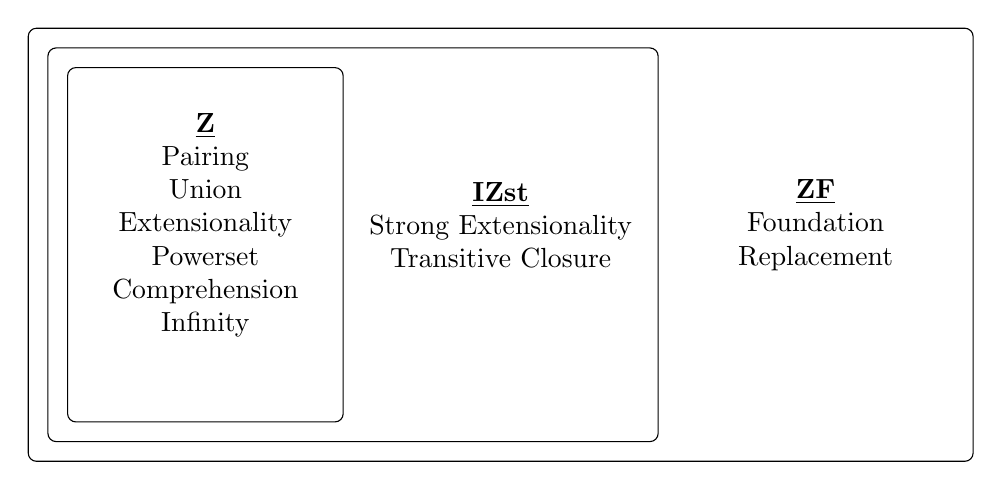
\begin{tikzpicture}[>=stealth,yscale=1,xscale=1]  

\draw[rounded corners=3pt] (0.5,0.5) rectangle (4,5);
\draw[rounded corners=3pt] (0.25,0.25) rectangle (8,5.25);
\draw[rounded corners=3pt] (0,0) rectangle (12,5.5);

\node(a) at (2.25,3)[text width=3cm,text centered] {\underline{\textbf{Z}} \\ Pairing \\ Union \\ Extensionality \\ Powerset \\ Comprehension \\ Infinity};
\node(b) at (6,3)[text width=10cm,text centered] {\underline{\textbf{IZst}} \\ Strong Extensionality \\ Transitive Closure};
\node(c) at (10,3)[text width=3cm,text centered] {\underline{\textbf{ZF}} \\ Foundation \\ Replacement};

\end{tikzpicture}
\end{center}

\section{The Language of Pointed Graphs}

\subsection{Sorts}

There are four sorts in IZmod \cite[see Section 3.2]{zermodulo}: graphs, nodes, classes of nodes and binary relations between nodes. We implemented the first two via the standard technique~\cite{theoryU} of defining a universe $\Set:\Type$ of sorts, a function $\El$ of type $\Set \ra \Type$ and two constants $graph$ and $node$ of type $\Set$:
\begin{lstlisting}
constant symbol graph : Set;
constant symbol node : Set;
\end{lstlisting}
We also introduce a constant $\arr $ of type $\Set \ra \Set \ra \Set$, together with its associated rewrite rule $\El~(x~\arr~y) \lra (\El~x) \ra (\El~y)$.

Contrary to deduction modulo, classes of nodes and binary relations on nodes can be expressed primitively via quantifications on propositions in \lpcm. The sort of classes is defined in \dedukti ~as $\El~node \ra \El~prop$ and that of binary relations as $\El~node \ra \El~node \ra \El~prop$.

The symbols $graph$ and $node$ are specific to the expression of IZmod in \dedukti, while in contrast the symbols $\Set$, $\El$ and $prop$ are part of the standard library of \dedukti.

\subsection{Signature}

The signature of IZmod contains 31 symbols \cite[see Table 2]{zermodulo}. As we have replaced the sorts for classes and relations with primitive \dedukti ~types, we do not need specific predicate symbols $mem$ and $rel$ to apply a class to a node or a relations to two. By virtue of the encoding of classes of nodes as elements of $\El~node \ra \El~prop$, $mem(x,P)$ can simply be expressed as $P~x$, and similarly $rel(x,y,r)$ can simply be expressed as $r~x~y$. In the same way, we do not need symbols $g_{x,y_1,...,y_n,P}$ and $g'_{x,x',y_1,...,y_n,P}$ to build classes and relations. Finally, the equality symbol is part of the standard library of \dedukti. The signature is thus reduced to 26 symbols. Below are the first 25 symbols, the specific case of the comprehension symbol is treated later.

\begin{lstlisting}
symbol eta : El graph → El node → El node → El prop;
symbol root : El graph → El node;
symbol cr : El graph → El node → El graph; // change of root

constant symbol o : El node;
symbol i : El node → El node;
symbol i' : El node → El node;
symbol j : El node → El node;
symbol j' : El node → El node;
symbol I : El node → El prop;
symbol J : El node → El prop;

// injection from graphs to nodes (for powerset) and its inverse
symbol ρ : El graph → El node;
symbol ρ' : El node → El graph;

// natural numbers
constant symbol O : El node;
symbol Succ : El node → El node;
symbol Pred : El node → El node;
symbol Null : El node → El prop;
symbol Nat : El node → El prop;
symbol < : El node → El node → El prop;

symbol simeq : El graph → El graph → El prop; // bisimilarity
symbol ∈ : El graph → El graph → El prop;
symbol join : El graph → El graph;
symbol pair : El graph → El graph → El graph;
symbol powerset : El graph → El graph;
symbol omega : El graph; // set of natural numbers
symbol closure : El graph → El graph;
\end{lstlisting}

\subsection{Rewriting Rules}

Among the rewrite rules \cite[see Table 3]{zermodulo}, we can drop the compatibility of equality with $mem$ as it comes for free with the Leibniz equality of \dedukti's standard library. We can also drop the rewrite rules determining the behavior of $g_{x,y_1,...,y_n,P}$ and $g'_{x,x',y_1,...,y_n,P}$, as they are superseeded by our encoding of classes and binary relations. The remaining rewrite rules are easy to implement in \dedukti:
\filbreak
\begin{center}
\underline{\textbf{General}}
\end{center}
\begin{lstlisting}
rule eta (cr $a $z) $x $y ↪ eta $a $x $y;
rule root (cr $a $x) ↪ $x;
rule (cr (cr $a $x) $y) ↪ cr $a $y;
\end{lstlisting}
\filbreak
\begin{center}
\underline{\textbf{Relocations}}
\end{center}
\begin{lstlisting}
rule i' (i $x) ↪ $x;
rule j' (j $x) ↪ $x;
rule ρ' (ρ $x) ↪ $x;
rule I (i $x) ↪ ⊤;
rule J (j $x) ↪ ⊤;
rule I (j $x) ↪ ⊥;
rule J (i $x) ↪ ⊥;
rule I (o) ↪ ⊥;
rule J (o) ↪ ⊥;

rule Pred (Succ $x) ↪ $x ;
rule Null O ↪ ⊤;
rule Nat O ↪ ⊤;
rule Null (Succ $x) ↪ ⊥;
rule Nat (Succ $x) ↪ Nat $x;

rule $x < O ↪ ⊥;
rule $x < (Succ $y) ↪ ($x < $y) ∨ ($x = $y);
\end{lstlisting}
\filbreak
\begin{center}
\underline{\textbf{Equality and Membership}}
\end{center}
\begin{lstlisting}
rule $a simeq $b ↪ `∃ r : El (node arrow (node arrow prop)), 
    r (root $a) (root $b)
    ∧ (`∀ x, `∀ x', `∀ y, 
        eta $a x' x ∧ r x y
            ⇒ `∃ y', eta $b y' y ∧ r x' y')
    ∧ (`∀ y, `∀ y', `∀ x, 
        eta $b y' y ∧ r x y
            ⇒ `∃ x', eta $a x' x ∧ r x' y');

rule $a ∈ $b ↪ `∃ x, ((eta $b x (root $b)) ∧ ($a simeq cr $b x));
\end{lstlisting}
\filbreak
\begin{center}
\underline{\textbf{Constructions}}
\end{center}
\begin{lstlisting}
rule eta (join $a) $x $x' ↪ 
	(`∃ y, `∃ y', ($x = i y) ∧ ($x' = i y') ∧ eta $a y y')
    ∨ (`∃ y, `∃ z, ($x = i y) 
    	∧ ($x' = o) 
    	∧ eta $a y z 
    	∧ eta $a z (root $a));

rule eta (pair $a $b) $x $x' ↪ 
	(`∃ y, `∃ y', (($x = i y) ∧ ($x' = i y') ∧ eta $a y y'))
    ∨ (`∃ y, `∃ y', ($x = j y) ∧ ($x' = j y') ∧ eta $b y y')
    ∨ (($x = i (root $a)) ∧ ($x' = o))
    ∨ (($x = j (root $b)) ∧ ($x' = o));

rule eta (powerset $a) $x $x' ↪ 
	(`∃ y, `∃ y', ($x = i y) ∧ ($x' = i y') ∧ eta $a y y')
    ∨ (`∃ y, `∃ c, ($x = i y) 
    	∧ ($x' = j (ρ c)) 
    	∧ (eta $a y (root $a)) 
    	∧ ((cr $a y) ∈ c))
    ∨ (`∃ c, ($x = j (ρ c)) ∧ ($x' = o));

rule eta omega $x $x' ↪ 
	(`∃ y, `∃ y', ($x = i y) ∧ ($x' = i y') ∧ (y < y'))
    ∨ (`∃ y, ($x = i y) ∧ ($x' = o) ∧ Nat y);

rule eta (closure $a) $x $x' ↪ 
	(`∃ y, `∃ y', (($x = i y) ∧ ($x' = i y') ∧ eta $a y y'))
	∨ (`∃ y, ($x = i y) 
        ∧ ($x' = o)
        ∧ (`∀ c : El (node arrow prop), 
                ((`∀ z, eta $a z (root $a) ⇒ c z)
                ∧ (`∀ z, `∀ z', (eta $a z z') ∧ (c z') ⇒ (c z)))
            ⇒ c y));
            
rule root (join $a) ↪ o;
rule root (pair $a $b) ↪ o;
rule root (powerset $a) ↪ o;
rule root omega ↪ o;
rule root (closure $a) ↪ o;
\end{lstlisting}

The pointed graph \texttt{omega} represents the set of Von Neumann ordinals \cite[see Table 2]{zermodulo}. Indeed, the rewriting rule of \texttt{eta omega x x'} states that in \texttt{omega} the edges correspond to the order relation $<$ and that there is an edge from every natural number to the root of \texttt{omega}. Therefore, the elements of \texttt{omega} are the natural numbers, and the elements of some natural number are all the natural numbers stricly below it, which corresponds to the definition of Von Neumann ordinals.


\section{The Language of Formulas}

This section is devoted to the operator that builds sets by comprehension. Indeed, in IZmod, the only valid sets of the form $\{x\in a\,|\,P(x)\}$ are those for which $P$ does not contain elements specific to the implementation of sets as pointed graphs, that is, all quantifiers in $P$ must be on $graph$ and $P$ can only use symbols $\in$, $\simeq$ and the logical connectives \cite[see Table 5]{zermodulo}. Taking this restriction into account is the main challenge of our implementation. In order to achieve this goal, we define a datatype representing the class of formulas just described, as well as an interpretation of this datatype into $El~prop$.

\subsection{Formulas}

We define the constant $formula$ of type $\Set$ and the operators for building elements of $El~formula$. Variables are represented as natural numbers and we do not need to handle $\alpha$-conversion as we do not need substitution.

\begin{lstlisting}
constant symbol formula : Set;
constant symbol eqF : El nat → El nat → El formula;
constant symbol inF : El nat → El nat → El formula;
constant symbol andF : El formula → El formula → El formula;
constant symbol orF : El formula → El formula → El formula;
constant symbol allF : El nat → El formula → El formula;
constant symbol exF : El nat → El formula → El formula;
constant symbol impF : El formula → El formula → El formula;
constant symbol fF : El formula;
constant symbol tF : El formula;
\end{lstlisting}

We also define an induction principle over formulas:

\begin{lstlisting}
constant symbol recF : Π (P : El formula → Prop), 
π(`∀ x, `∀ y, P (eqF x y))
→ π(`∀ x, `∀  y, P (inF x y))
→ π(`∀ f, `∀ g, (P f ∧ P g) ⇒ (P (andF f g)))
→ π(`∀ f, `∀ g, (P f ∧ P g) ⇒ (P (orF f g)))
→ π(`∀ f, `∀ g, (P f ∧ P g) ⇒ (P (impF f g)))
→ π(`∀ f, (P f) ⇒ (`∀ x, P (allF x f)))
→ π(`∀ f, (P f) ⇒ (`∀ x, P (exF x f)))
→ π(P tF)
→ π(P fF)
→ π(`∀ f, P f);
\end{lstlisting}

\subsection{Interpretation}

In this section, we define the interpretation of the datatype of formulas into the type of propositions. Since formulas can contain variables (represented as natural numbers), the interpretation depends on a valuation from natural numbers to graphs. Hence we have:

\begin{lstlisting}
symbol interpretation : (El nat → El graph) → El formula → El prop;
\end{lstlisting} 

The interpretation of quantifiers requires an operator for updating a valuation, taking as arguments the initial valuation, the variable that needs to be updated, and the new value of this variable:

\begin{lstlisting}
symbol update : (El nat → El graph) → El nat → El graph
                                         → (El nat → El graph)
\end{lstlisting} 

The computation of $update~\sigma~x~a~y$ relies on a decision procedure for the equality on natural numbers: if $x=y$ then $update~\sigma~x~a~y$ is $a$, other wise it is $\sigma~y$. Rather than implementing such a decision procedure separately, we embed it in an auxiliary function:

\begin{lstlisting}
symbol update1 : (El nat → El graph) → El nat → El graph → El nat
                                         → (El nat → El graph)
\end{lstlisting} 

$update~\sigma~x~a~y$ reduces to $update1~\sigma~x~a~y~y$, and $update1~\sigma~x~a~y~z$ reduces to $a$ if $x=y$, and $\sigma~z$ otherwise, by decreasing $x$ and $y$ until one (or both) becomes $zero$. The last argument to $update1$ is thus used for storing the variable at which $update~\sigma~x~a$ was initially called. The rewrite rules are as follows:

\begin{lstlisting}
rule update $σ $x $a $y ↪ update1 $σ $x $a $y $y;
rule update1 $σ zero $a zero $z ↪ $a;
rule update1 $σ zero $a (s $y) $z ↪ $σ $z;
rule update1 $σ (s $x) $a zero $z ↪ $σ $z;
rule update1 $σ (s $x) $a (s $y) $z ↪ update1 $σ $x $a $y $z;
\end{lstlisting}

We can prove that $update$ and $update1$ satisfy the intended properties:

\begin{theorem}
\begin{equation*}
\begin{split}
\fa \sigma \fa x \fa y \fa z \fa a ~((x = y \ \imp \ update1 \ \sigma \ x \ a \ y \ z \ = \ a) \ \conj \ (\blneg \ x = y \ \imp \ update1 \ \sigma \ x \ a \ y \ z \ = \ \sigma \ z))
\\
\fa \sigma \fa \sigma' \fa x \fa a \fa b~ (a \ \simeq \ b \ \imp \ (\fa y~ (\sigma \ y \ \simeq \ \sigma' \ y)) \ \imp \ \fa z~ (update \ \sigma \ x \ a \ z \ \simeq \ update \ \sigma' \ x \ b \ z))
\end{split}
\end{equation*}
\end{theorem}

Now we have all the tools to define the rewriting rules of the interpretation of formulas:

\begin{lstlisting}
rule interpretation $σ (eqF $x $y) ↪ ($σ $x) simeq ($σ $y);
rule interpretation $σ (inF $x $y) ↪ ($σ $x) ∈ ($σ $y);
rule interpretation $σ (andF $f $g)
                ↪ (interpretation $σ $f) ∧ (interpretation $σ $g);
rule interpretation $σ (orF $f $g)
                ↪ (interpretation $σ $f) ∨ (interpretation $σ $g);
rule interpretation $σ (impF $f $g)
                ↪ (interpretation $σ $f) ⇒ (interpretation $σ $g);
rule interpretation $σ (allF $x $f)
                ↪ `∀ a, interpretation (update $σ $x a) $f;
rule interpretation $σ (exF $x $f)
                ↪ `∃ a, interpretation (update $σ $x a) $f;
rule interpretation $σ fF ↪ ⊥;
rule interpretation $σ tF ↪ ⊤;
\end{lstlisting}

We can finally prove that $interpretation$ is invariant under $\simeq$-equivalent valuations:

\begin{theorem}
$\fa f \fa \sigma \fa \sigma' ~((interpretation \ \sigma \ f \ \conj \ \fa x ~(\sigma \ x \ \simeq \ \sigma' \ x)) \ \imp \ interpretation \ \sigma' \ f)$
\end{theorem}
\begin{proof}
By induction over formula f. $\square$
\end{proof}

\subsection{Comprehension, Empty Set and Inductive Set}

With this syntax for restricted formulas at hand together with the interpretation in $prop$, we are finally able to define the comprehension construction in \dedukti:

\begin{lstlisting}
symbol comp : El graph → (El nat → El graph) → El formula
                                                       → El graph;
\end{lstlisting}

together with its rewrite rules

\begin{lstlisting}
rule eta (comp $a $σ $f) $x $x' ↪ 
	(`∃ y, `∃ y', (($x = i y) ∧ ($x' = i y') ∧ eta $a y y')) 
	∨ (`∃ y, ($x = i y) ∧ ($x' = o) ∧ (eta $a y (root $a))
	∧ (interpretation (update $σ zero (cr $a y)) $f));
rule root (comp $a $σ $f) ↪ o;
\end{lstlisting}

When it comes to the symbol related to the Infinity section of \cite[see Section 2.1]{zermodulo}, we implement $empty\_set$ of type $\El~graph$ and $Ind$ of type $\El~graph \ \ra \ \El~prop$.

Using comprehension with the set of natural numbers and the formula $fF$ gives the empty set:
\begin{lstlisting}
rule empty_set ↪ comp omega (λ _, omega) fF;
\end{lstlisting}

and we can define inductive sets:

\begin{lstlisting}
rule Ind $c ↪ (empty_set ∈ $c) 
∧ (`∀ a, (a ∈ $c) ⇒ ((join (pair a (pair a a))) ∈ $c));
\end{lstlisting}

\section{Lemmas}

Dowek and Miquel proved that the theory IZmod of pointed graph does validate all the axioms of IZst. This required 53 lemmas that were \textit{informally} proved~\cite[see Tables 4 and 5]{zermodulo} and that we prove \textit{formally} in our implementation. Some of our proofs just follow the informal ones, while some others rely on the type of formulas and its embedding into propositions. 

The first two lemmas are immediate consequences of the definition of Leibniz equality in the standard library of \dedukti:
\begin{lstlisting}
constant symbol = [s] : El s → El s → El prop;
notation = infix 4;
rule π (@= $s $x $y) ↪ Π (P : El $s → El prop), π(P $x) → π(P $y);
\end{lstlisting}

All the other lemmas of IZmod not involving $comp$ (and therefore restricted formulas) are proved using the blueprint~\cite[see Proposition 1]{zermodulo53}. The complete proofs can be found in \url{https://github.com/Deducteam/dedukti_set_theory/}.

\subsection{An Example of Proof}

To show the way lemmas are proved in \dedukti ~we will take the example of lemma 30 and comment its proof. This lemma states that $$ a \in b \conj a \simeq c \imp c \in b $$

\begin{proof}
We first assume graphs $a$, $b$ and $c$ and $H$ the proof of $ a \in b \conj a \simeq c $. $a \in b$ rewrites to $\ex x~(x~\eta_b~root~b \conj a \simeq (b/x))$. 

We decompose the left part of $H$ as $x$ and $Hx$ which is a proof of $x~\eta_b~root~b \conj a \simeq (b/x)$. 

As the goal is to prove $c \in b$, that is, $\ex y~(y~\eta_b~root~b \conj c \simeq (b/y))$, we need to find a suitable $y$. We take $x$ and now have two goals: $x~\eta_b~root~b$ and $c \simeq (b/x)$. 

The first one is proved by applying the left part of $Hx$. 

The second one is obtained by applying lemma 5 (transitivity of $\simeq$) to $c$, $a$ and $b/x$. To apply lemma 5, we need to prove $c \simeq a \conj a \simeq b/x$. $c \simeq a$ is proved by applying lemma 4 (symmetry of $\simeq$) to $a$, $c$ and the right part of $H$ that is a proof of $a \simeq c$. $a \simeq b/x$ derives from the right part of $Hx$. $\square$
\end{proof}

This proof is written in \dedukti ~with the following code: 

\begin{lstlisting}
opaque symbol lemma30 : π(`∀ a, `∀ b, `∀ c, 
	((a ∈ b) ∧ (a simeq c)) ⇒ (c ∈ b))
≔ begin
assume a b c H;
refine ex_e node _ (and_el _ _ H) _ _;
assume x Hx;
refine ex_i node x _ _;
refine and_i _ _ _ _
{refine and_el _ _ Hx}
{refine lemma5 c a (cr b x) 
	(and_i _ _ (lemma4 a c (and_er _ _ H)) (and_er _ _ Hx))}
end;
\end{lstlisting}

\subsection{Lemmas involving Formulas}

Lemma 32 is as follows:

$$(P(z \leftarrow a) \conj a \simeq b) \imp P(z \leftarrow b)$$

where $P$ is a restricted formula. Therefore, we formulate lemma 32 using the type of formulas, as well as its interpretation in $prop$. The valuation $update~\sigma~z~a$ represents the assignment of variable $z \leftarrow a$.

\begin{lstlisting}
opaque symbol lemma32 : Π (z : El nat), Π (f : El formula), 
	π(`∀ a, `∀ b, (`∀ σ : (El nat → El graph),
	((interpretation (update σ z a) f) ∧ (a simeq b)) 
	⇒ (interpretation (update σ z b) f)))
\end{lstlisting}

The proof proceeds by induction over formulas: each case is proved easily, using the lemmas that have already been checked by \dedukti. \\

Lemma 41 is implemented similarly:

\begin{lstlisting}
opaque symbol lemma41 : Π (x y : El nat), Π (f : El formula), 
	Π (c d : El graph), π(`∀ σ : (El nat → El graph), 
	((interpretation (update (update σ x c) y d) f)
	∧ (`∀ a, `∀ a', `∀ b, 
		((a' ∈ a) 
		∧ (interpretation (update (update σ x a) y b) f)) 
		⇒ (`∃ b', ((b' ∈ b) 
			∧ (interpretation (update (update σ x a') y b') f))))
	∧ (`∀ b, `∀ b', `∀ a, 
		((b' ∈ b) 
		∧ (interpretation (update (update σ x a) y b) f)) 
		⇒ (`∃ a', ((a' ∈ a) 
			∧ (interpretation (update (update σ x a') y b') f))))) 
	⇒ (c simeq d))
\end{lstlisting}

\subsection{Weak Extensionnality}

\label{extensionality}

The proofs of lemmas 44, 47 and 48 require the use of the axiom of (weak) extensionality~\cite{zermodulo53}. Therefore, we prove in \dedukti ~that extensionality is a consequence of strong extensionality (lemma 41):\\

\textbf{Weak extensionality.} $\fa c\fa d~ (\fa z~ (z \in c \Leftrightarrow z \in d) \imp c \simeq d)$ \\


\begin{proof}
We assume that $\fa z~ (z \in c \Leftrightarrow z \in d)$. In order to prove $c \simeq d$, we follow the blueprint given by Dowek and Miquel~\cite[see Proposition 1]{zermodulo} by using an instance of the strong extensionality axiom where $R(x,y)$ is $(x \simeq c~\conj~y \simeq d)~\disj~x \simeq y$. We are left to prove the three premises of this instance of strong extensionality:
\begin{itemize}
\item $(c \simeq c~\conj~d \simeq d)~\disj~c \simeq d$ is a tautology.
\item We need to prove:
$$\fa a\fa a'\fa b~(a' \in a~\conj~((a \simeq c~\conj~b \simeq d)~\disj~a \simeq b) \imp (\ex b'~ (b' \in b~\conj~((a' \simeq c~\conj~b' \simeq d)~\disj~a' \simeq b'))$$
We assume $(a' \in a~\conj~((a \simeq c~\conj~b \simeq d)~\disj~a \simeq b)$ and we choose $b'$ equal to $a'$, so that $(a' \simeq c~\conj~a' \simeq d)~\disj~a' \simeq a'$ is a tautology and we are left to prove $a' \in b$. If $a \simeq b$, then by lemma 31 this is a consequence of $a' \in a$. Otherwise we have $a \simeq c~\conj~b \simeq d$ so with lemma 31 applied twice we are left to prove $a' \in c \imp a' \in d$, which is a consequence of $\fa z~ (z \in c \Leftrightarrow z \in d)$.
\item We proceed similarly for the third premise. $\square$
\end{itemize}
\end{proof}

In order to implement this result in \dedukti ~we first prove the following intermediary lemma:

\begin{lstlisting}
opaque symbol lemmaHypExt : Π (c d : Graph), 
	π((`∀ z, (z ∈ c) ⇔ (z ∈ d)) ⇒ 
	((((c simeq c) ∧ (d simeq d)) ∨ (c simeq d))
	∧ (`∀ a, `∀ a', `∀ b, 
		((a' ∈ a) ∧ (((a simeq c) ∧ (b simeq d)) ∨ (a simeq b))) 
		⇒ (`∃ b', ((b' ∈ b) 
		∧ (((a' simeq c) ∧ (b' simeq d)) ∨ (a' simeq b')))))
	∧ (`∀ b, `∀ b', `∀ a, 
		((b' ∈ b) ∧ (((a simeq c) ∧ (b simeq d)) ∨ (a simeq b)))
		 ⇒ (`∃ a', ((a' ∈ a) 
	 	∧ (((a' simeq c) ∧ (b' simeq d)) ∨ (a' simeq b')))))))
\end{lstlisting}

Then in order to prove $weak \ extensionality$, we assume graphs $c$ and $d$, and $H$ the hypothesis $\fa z~ (z \in c) \Leftrightarrow (z \in d)$. Then we apply lemma 41 to:

\begin{itemize}
\item natural numbers $zero$ and $one$
\item the formula $(orF~(andF~(eqF~zero~two)~(eqF~one~three))~(eqF~zero~one))$
\item graphs $c$ and $d$
\item the valuation $(update~(update~(\lambda \_, empty\_set)~two~c)~three~d)$ 
\item the proof $lemmaHypExt~c~d~H$.
\end{itemize}

Indeed, in the formula $(orF~(andF~(eqF~zero~two)~(eqF~one~three))~(eqF~zero~one))$, $two$ will be interpreted by $c$ and $three$ by $d$, thanks the valuation $(update~(update~(\lambda \_, empty\_set)~two~c)~three~d)$. Finally we obtain:


\begin{lstlisting}
opaque symbol lemmaExt : Π (c d : El graph), 
	π((`∀ x, (x ∈ c) ⇔ (x ∈ d)) ⇒ (c simeq d))
≔ begin
assume c d H;
refine lemma41 zero one 
	(orF (andF (eqF zero two) (eqF one three)) (eqF zero one)) 
	c d (update (update (λ _, empty_set) two c) three d) 
	(lemmaHypExt c d H)
end;
\end{lstlisting}

\subsection{The Axioms of IZst Theory}

We have now encoded in \dedukti ~all the axioms of IZst set theory: the strong extensionality axiom corresponds to lemma 41, the axiom of the union is implemented by lemma 42, the pairing axiom corresponds to lemma 43, the axiom of the power set is encoded by lemma 44, the comprehension scheme is implemented by lemma 45, the axiom of infinity corresponds to lemma 51 and the transitive closure axiom is encoded by lemmas 52 and 53.


\section{Conclusion}

We have implemented in \dedukti ~a version of set theory -- IZst -- that corresponds to Zermelo set theory, with the Strong Extensionality axiom and the Transitive Closure axiom. To do so, we have adapted the work by G. Dowek and A. Miquel \cite{zermodulo} from \textit{Deduction modulo theory} to \lpcm ~and have encoded sets with a structure of pointed graphs of the IZmod theory. We have \textit{formally} written all the proofs of the lemmas allowing us to implement set theory in \dedukti.

To define and prove the lemmas corresponding to the Comprehension axiom, we have developed a language of formulas, along with operators \textit{interpretation} and \textit{update}. In particular, the language of formulas allows us to prove that the Extensionality axiom derives from the Strong Extensionality axiom.

Historically, the encoding of sets by pointed graphs had been designed to enjoy the normalization property. IZmod expressed in \textit{Deduction modulo theory} does so, but the case of our implementation in \lpcm ~remains to be investigated.

The implementation of IZmod theory represents a significant corpus of formal proofs in \textsc{Lambdapi}.

\newpage
\section*{Annex}

\begin{center}
\begin{tabular}{|c|c||c|c|}
\hline Lemma & Number of lines in the proof & Lemma & Number of lines in the proof \\
\hline 3 & 26 & 29 & 17 \\
\hline 4 & 14 & 30 & 10 \\
\hline 5 & 37 & 31 & 12 \\
\hline 6 & 33 & 32 & 49 \\
\hline 7 & 12 & 33 & 33 \\
\hline 8 & 5 & 34 & 33 \\
\hline 9 & 12 & 35 & 9 \\
\hline 10 & 12 & 36 & 9 \\
\hline 11 & 5 & 37 & 9 \\
\hline 12 & 5 & 38 & 9 \\
\hline 13 & 5 & 39 & 9 \\
\hline 14 & 37 & 40 & 9 \\
\hline 15 & 40 & 41 & 42 \\
\hline 16 & 48 & Weak extensionality & 47 \\
\hline 17 & 48 & 42 & 49 \\
\hline 18 & 38 & 43 & 39 \\
\hline 19 & 44 & 44 & 133 \\
\hline 20 & 90 & 45 & 46 \\
\hline 21 & 34 & 46 & 11 \\
\hline 22 & 35 & 47 & 18 \\
\hline 23 & 34 & 48 & 165 \\
\hline 24 & 38 & 49 & 11 \\
\hline 25 & 31 & 50 & 23 \\
\hline 26 & 38 & 51 & 6 \\
\hline 27 & 29 & 52 & 17 \\
\hline 28 & 33 & 53 & 31 \\
\hline
\end{tabular}
\end{center}




%\nocite{*}
\bibliographystyle{eptcs}
\bibliography{biblio}
\end{document}
